\begin{figure}[H]
\centering
\includegraphics[page=1,width=0.44\textwidth]{\FCNCFigures/tthML/raw/faketau/prefit/NOMINAL/reg1l1tau1b1j_ss_vetobtagwp70_highmet/tau_pt_0.pdf}
%\put(-100, 140){\textbf{(a)}}
\put(-120, 100){\footnotesize{Fake/Real tau inclusive.}}
\includegraphics[page=1,width=0.44\textwidth]{\FCNCFigures/tthML/raw/faketau/prefit/NOMINAL/reg1l1tau1b2j_ss_vetobtagwp70_highmet/tau_pt_0.pdf}
%\put(-100, 140){\textbf{(b)}}
\put(-120, 100){\footnotesize{Fake/Real tau inclusive.}}

\includegraphics[page=1,width=0.44\textwidth]{\FCNCFigures/tthML/raw/faketau/prefit/NOMINAL/reg1l1tau1b2j_os_vetobtagwp70_highmet/tau_pt_0.pdf}
%\put(-100, 140){\textbf{(c)}}
\put(-120, 100){\footnotesize{Fake/Real tau inclusive.}}
\includegraphics[page=1,width=0.44\textwidth]{\FCNCFigures/tthML/raw/faketau/prefit/NOMINAL/reg1l1tau1b3j_os_vetobtagwp70_highmet/tau_pt_0.pdf}
%\put(-100, 140){\textbf{(d)}}
\put(-120, 100){\footnotesize{Fake/Real tau inclusive.}}

\includegraphics[page=1,width=0.44\textwidth]{\FCNCFigures/tthML/raw/faketau/prefit/NOMINAL/reg1l2tau1bnj_os/tau_pt_0.pdf}
%\put(-100, 140){\textbf{(e)}}
\put(-120, 100){\footnotesize{Fake/Real tau inclusive.}}

\caption{ The distributions of $\tau$ $\pt$ in the signal regions in leptonic channel. The samples shown in these figures are fake/real tau inclusive.The yields shown in these
figures are the sum of fake and real taus from each sample. Only statistical uncertainties are being shown. Underflow and overflow bins are included respectively in the first and last bins. Empty data bins here are always blinded based on our strategy.}

\label{fig:pt_raw}
\end{figure}
